\documentclass[12pt,a4paper]{article}
\usepackage[utf8]{inputenc}
\usepackage{amsmath}
\usepackage{amsfonts}
\usepackage{amssymb}
\usepackage{graphicx}
\usepackage{makecell}
\usepackage[font=small,labelfont=bf]{caption}

\renewcommand\theadalign{bc}
\renewcommand\theadfont{\bfseries}
\renewcommand\theadgape{\Gape[4pt]}
\renewcommand\cellgape{\Gape[4pt]}
\graphicspath{ {images/} }

\author{Isaac Ashwin Ravindran}
\date{1002151}
\title{CSE Network Security Lab 1}
\begin{document}
	\pagenumbering{gobble}
	\maketitle
	\newpage
	\pagenumbering{arabic}
	
	\section{Measurement of Round Trip Times using Ping}
		\subsection{Question 1}
		For each host, record the percentage of packets sent that resulted in a successful response. Record also the minimum, average, and maximum round trip times for the packets that resulted in a response.
	
		\begin{center}
			\begin{tabular}{||c c c c c||} 
 				\hline
				\thead{Location} & \thead{Successful \\ Percentage} & \thead{Min \\ RTT (ms)} & \thead{Average \\ RTT (ms)} & \thead{Max \\ RTT (ms)} \\
 				\hline\hline
 				www.csail.mit.edu & 100\% & 4.039 & 5.888 & 10.466 \\ 
 				\hline
 				www.berkeley.edu & 100\% & 202.702 & 294.037 & 398.142 \\ 
 				\hline
				www.usyd.edu.au & 100\% & 143.507 & 200.593 & 305.575 \\ 
 				\hline
				www.kyoto-u.ac.jp & 100\% & 78.128 & 102.966 & 201.455 \\ 
 				\hline
			\end{tabular}
		\end{center}
		
		\subsection{Question 2}
			\paragraph{Describe and explain the differences in the minimum round trip time to each of these hosts.}
			\begin{itemize}
				\item \verb|www.csail.mit.edu| - MIT makes use of Pantheon to host their website. It provides distributed hosting across the world, therefore giving very low pings from anywhere. Hence, it has the lowest ping of the lot. 
				\item \verb|www.berkeley.edu| - As this university's website is located in the US, the data needs to travel a very long geographical distance to reach Singapore, therefore resulting in very high ping times.
				\item \verb|www.usyd.edu.au| - This university, being located in Australia, is closer than Berkeley. Therefore, while high, it's ping times are still lower than Berkeley.
				\item \verb|www.kyoto-u.ac.jp| - Kyoto University is in Japan, which is still in the same continent and therefore is much closer than the previous 2 universities. Therefore it has the shortest time out of the last 3.
			\end{itemize}
		
		\newpage
		
		\subsection{Question 3}
		Repeat the exercise using packet sizes of 56, 512 and 1024 bytes. Record the minimum, average, and maximum round trip times for each of the packet sizes.
	
		\begin{center}
			\begin{tabular}{||c c c c c c||} 
 				\hline
				\thead{Location} & \thead{Packet \\ Size (B)} & \thead{Successful \\ Percentage} & \thead{Min \\ RTT \\ (ms)} & \thead{Average \\ RTT \\ (ms)} & \thead{Max \\ RTT \\ (ms)} \\
 				\hline\hline
 				www.csail.mit.edu & 56 & 100\% & 4.039 & 5.888 & 10.466 \\ 
 				\hline
 				www.csail.mit.edu & 512 & 100\% & 4.835 & 12.877 & 32.240 \\ 
 				\hline
 				www.csail.mit.edu & 1024 & 0\% & - & - & - \\ 
 				\hline
 				www.berkeley.edu & 56 & 100\% & 202.702 & 294.037 & 398.142 \\ 
 				\hline
 				www.berkeley.edu & 512 & 100\% & 202.565 & 262.395 & 327.723 \\ 
 				\hline
 				www.berkeley.edu & 1024 & 0\% & - & - & - \\ 
 				\hline
				www.usyd.edu.au & 56 & 100\% & 143.507 & 200.593 & 305.575 \\ 
 				\hline
 				www.usyd.edu.au & 512 & 100\% & 198.095 & 271.715 & 362.179 \\ 
 				\hline
 				www.usyd.edu.au & 1024 & 0\% & - & - & - \\ 
 				\hline
				www.kyoto-u.ac.jp & 56 & 100\% & 78.128 & 102.966 & 201.455 \\ 
 				\hline
 				www.kyoto-u.ac.jp & 512 & 100\% & 93.773 & 138.465 & 220.646 \\ 
 				\hline
 				www.kyoto-u.ac.jp & 1024 & 0\% & - & - & - \\
 				\hline
			\end{tabular}
		\end{center}
		
		\paragraph{Why are the minimum round-trip times to the same hosts different when using 56, 512, and 1024–byte packets?}
		\paragraph{}
			The packets take longer to transmit due to the larger size. Therefore the larger the packet, the longer the minimum RTT.
			
		\newpage
		
		\subsection{Question 4}
			Use ping to send 100 packets to the following host. Each packet should have a size of 56 bytes, and there should be an interval of 5 seconds between each packet sent.
			\\
			\\
			\verb|www.wits.ac.za|
			\paragraph{Record the percentage of the packets sent that resulted in a successful response.}
			\paragraph{}
				0\%
			\paragraph{What are some possible reasons why you may not have received a response?}
			\paragraph{}
				It is possible that the sysadmin of the University of Witwatersand blocked ICMP on their routers. Therefore ICMP messages do not get sent out, resulting in no response when performing a \verb|ping|.
		\newpage
		
		\section{Understanding Internet Routes Using Traceroute}
			\subsection{Question 5}
				\paragraph{Explain how traceroute discovers a path to a remote host.}
				\paragraph{}
					\verb|traceroute| progressively sends packets with increasing TTLs (starting from 1) until it sends a packet that has a TTL that reaches the intended destination. This way, all intermediate routers/servers/computers will notify the original sender (\verb|traceroute| program) that the TTL has expired, allowing \verb|traceroute| to know all the hops along the way.
			
			\subsection{Question 6}
				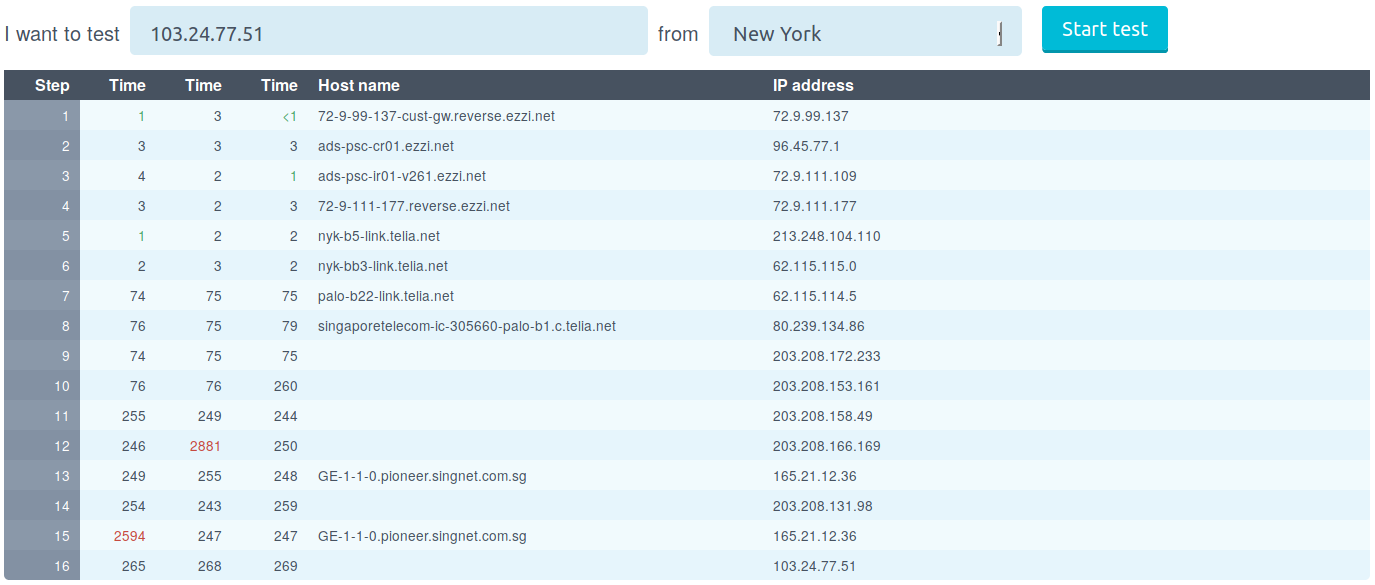
\includegraphics[scale=0.3]{fromnewyork}
				\captionof{figure}{ Traceroute from New York}
				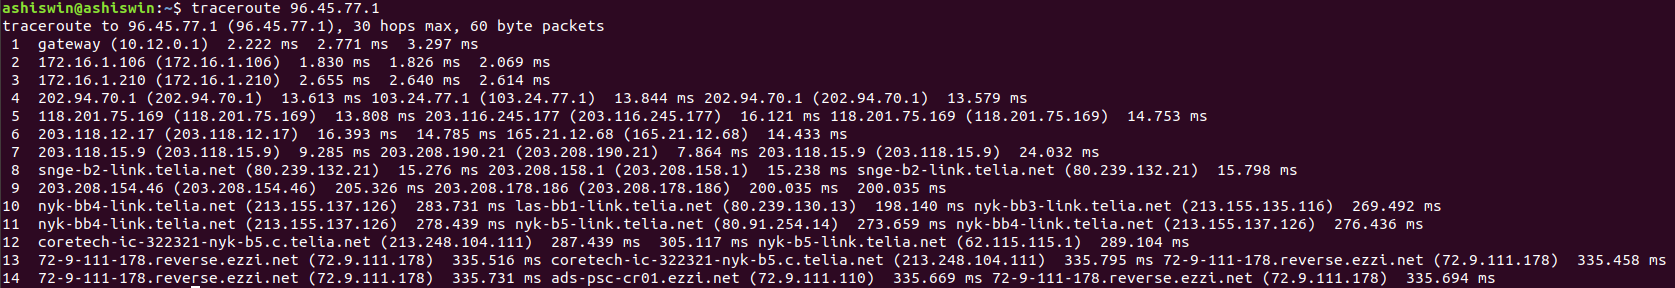
\includegraphics[scale=0.25]{tonewyork}
				\captionof{figure}{ Traceroute to New York}
				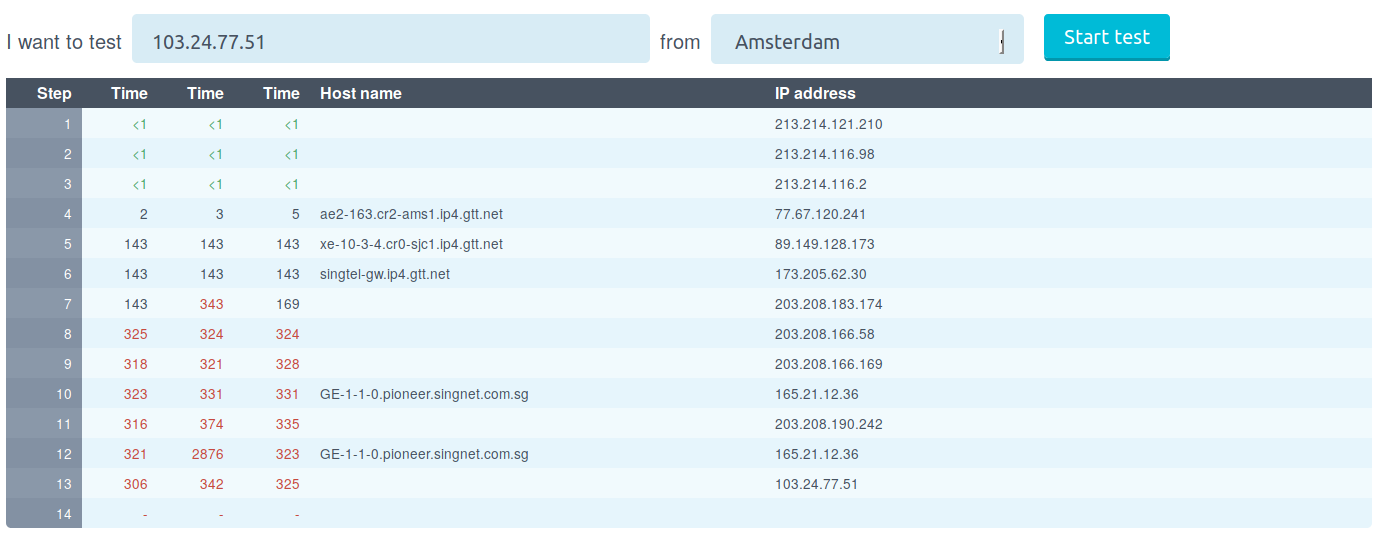
\includegraphics[scale=0.3]{fromamsterdam}
				\captionof{figure}{ Traceroute from Amsterdam}
				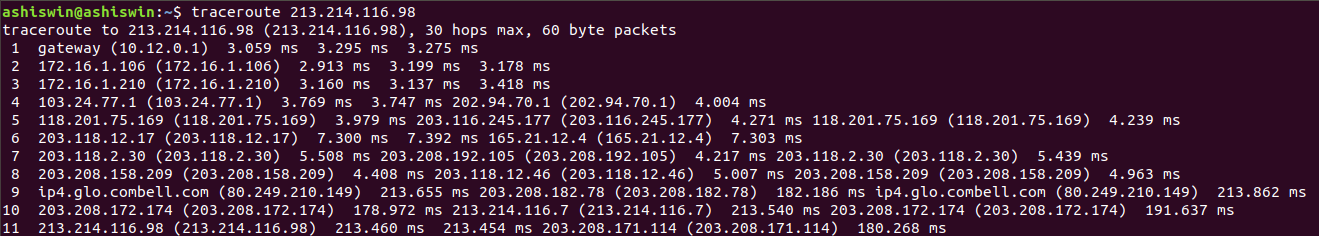
\includegraphics[scale=0.3]{toamsterdam}
				\captionof{figure}{ Traceroute to Amsterdam}
				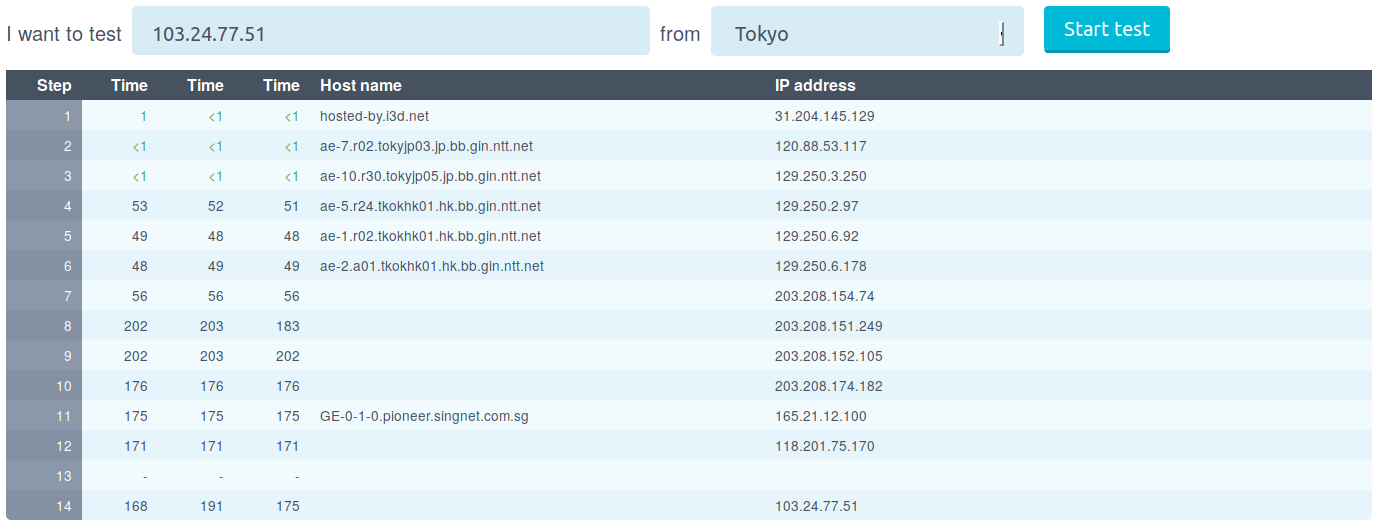
\includegraphics[scale=0.3]{fromtokyo}
				\captionof{figure}{ Traceroute from Tokyo}
				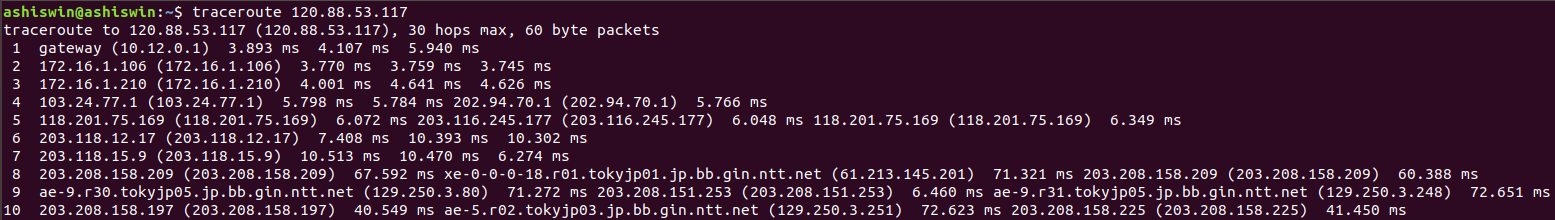
\includegraphics[scale=0.26]{totokyo}
				\captionof{figure}{ Traceroute to Tokyo}
			\subsection{Question 7}
				\paragraph{Describe anything unusual you might observe about the output. Are the same routers traversed in both directions? If no, why might this be the case?}
				\paragraph{}
					No, the same routers are not traversed in both directions. Usually, the incoming interface IP address is used in the ICMP error messages, so you see a different IP address while running \verb|traceroute| in different directions.
\end{document}